% A LaTeX (non-official) template for ISAE projects reports
% Copyright (C) 2014 Damien Roque
% Version: 0.2
% Author: Damien Roque <damien.roque_AT_isae.fr>

\documentclass{beamer}
\usepackage[utf8]{inputenc}
\usepackage[ngerman]{babel}
\usepackage{palatino}
\usepackage{graphicx}
\graphicspath{{./images/}}
\usepackage{colortbl}
\usepackage{xcolor}
\usepackage{tikz}
\usetikzlibrary{shapes,arrows}
\usetikzlibrary{mindmap,trees}
\usetikzlibrary{calc}
\usepackage{pgfplots}
\pgfplotsset{compat=newest}
\pgfplotsset{plot coordinates/math parser=false}
\newlength\figureheight
\newlength\figurewidth
\usepackage{ifthen}
\usepackage{subfigure}
\usepackage{amsthm}
\usepackage{amsfonts}
\usepackage{amssymb}
\usepackage{amsmath}
\usepackage{eurosym}
\usepackage{wasysym}

% Printing on 2 slides per page
%\pgfpagesuselayout{2 on 1}[a4paper,border shrink=5mm]

% My macros...
\newcommand*{\SET}[1]  {\ensuremath{\boldsymbol{#1}}}
\newcommand*{\VEC}[1]  {\ensuremath{\boldsymbol{#1}}}
\newcommand*{\MAT}[1]  {\ensuremath{\boldsymbol{#1}}}
\newcommand*{\OP}[1]  {\ensuremath{\text{#1}}}
\newcommand*{\NORM}[1]  {\ensuremath{\left\|#1\right\|}}
\newcommand*{\DPR}[2]  {\ensuremath{\left \langle #1,#2 \right \rangle}}
\newcommand*{\calbf}[1]  {\ensuremath{\boldsymbol{\mathcal{#1}}}}
\newcommand*{\shift}[1]  {\ensuremath{\boldsymbol{#1}}}
\newcommand{\eqdef}{\stackrel{\mathrm{def}}{=}}
\newcommand{\argmax}{\operatornamewithlimits{argmax}}
\newcommand{\argmin}{\operatornamewithlimits{argmin}}
\newcommand{\ud}{\, \text{d}}
\newcommand{\vect}{\text{Vect}}
\newcommand{\sinc}{\text{sinc}}
\newcommand{\esp}{\ensuremath{\mathbb{E}}}
\newcommand{\hilbert}{\ensuremath{\mathcal{H}}}
\newcommand{\fourier}{\ensuremath{\mathcal{F}}}
\newcommand{\sgn}{\text{sgn}}
\newcommand{\intTT}{\int_{-T}^{T}}
\newcommand{\intT}{\int_{-\frac{T}{2}}^{\frac{T}{2}}}
\newcommand{\intinf}{\int_{-\infty}^{+\infty}}
\newcommand{\Sh}{\ensuremath{\boldsymbol{S}}}
\newcommand{\Cpx}{\ensuremath{\mathbb{C}}}
\newcommand{\R}{\ensuremath{\mathbb{R}}}
\newcommand{\Z}{\ensuremath{\mathbb{Z}}}
\newcommand{\N}{\ensuremath{\mathbb{N}}}
\newcommand{\K}{\ensuremath{\mathbb{K}}}
\newcommand{\reel}{\mathcal{R}}
\newcommand{\imag}{\mathcal{I}}
\newcommand{\cmnr}{c_{m,n}^\reel}
\newcommand{\cmni}{c_{m,n}^\imag}
\newcommand{\cnr}{c_{n}^\reel}
\newcommand{\cni}{c_{n}^\imag}
\newcommand{\LR}{\mathcal{L}_2(\R)}
\newcommand{\tproto}{g}
\newcommand{\rproto}{\check{g}}
\newcommand{\Tproto}{G}
\newcommand{\Rproto}{\check{G}}

%\theoremstyle{definition}
%\newtheorem{definition}{Définition}[subsection]

\theoremstyle{remark}
\newtheorem{remarque}{Remarque}[subsection]

\theoremstyle{plain}
\newtheorem{propriete}{Propriété}[subsection]
\newtheorem{exemple}{Exemple}[subsection]

% Choosing a main theme and a color theme
\mode<presentation> {
  %\usetheme{Warsaw}
  \usetheme{Madrid}
  %\usetheme{Frankfurt}
  \usecolortheme{seahorse}
}


\addtobeamertemplate{frametitle}{}{%
\vskip-1em
\begin{tikzpicture}[remember picture,overlay]
\node[anchor=north east,yshift=4pt] at (current page.north east) {
\includegraphics[height=0.8cm]{images/logo-isae-long-sans-texte}};
\end{tikzpicture}}

\title[Recap keys \& console]{RMI Konzept Team 13}

\author[APPE Team 13]{\small Tobias Kreienbühl, Marco Moro, Severin Gmür, Ramon Wyss}

%\date{\today}

% Clear the navigation bar
\setbeamertemplate{navigation symbols}{}
 
%\subject{Sujet de la présentation}

\begin{document}

\begin{frame}
\titlepage
\end{frame}


\begin{frame}
  \frametitle{Plan}
  \small
  \tableofcontents
  \normalsize
\end{frame}

% Recall the outline at each section
\AtBeginSection[]
{%
\begin{frame}
  \frametitle{Ablauf}
  \small
  %\tableofcontents[hideothersubsections]
  \tableofcontents[currentsection,hideothersections]
  %\tableofcontents[currentsubsection]
  \normalsize
\end{frame}
}

\section{Remoteschicht ohne RMI}
% !TEX root = isae-beamer-template.tex

% Recall the outline at each section
\begin{frame}
  \frametitle{Remoteschicht ohne RMI}
	    \begin{column}{1\linewidth}
	    	Beispiel Artikel:
	    	\begin{center}
	    		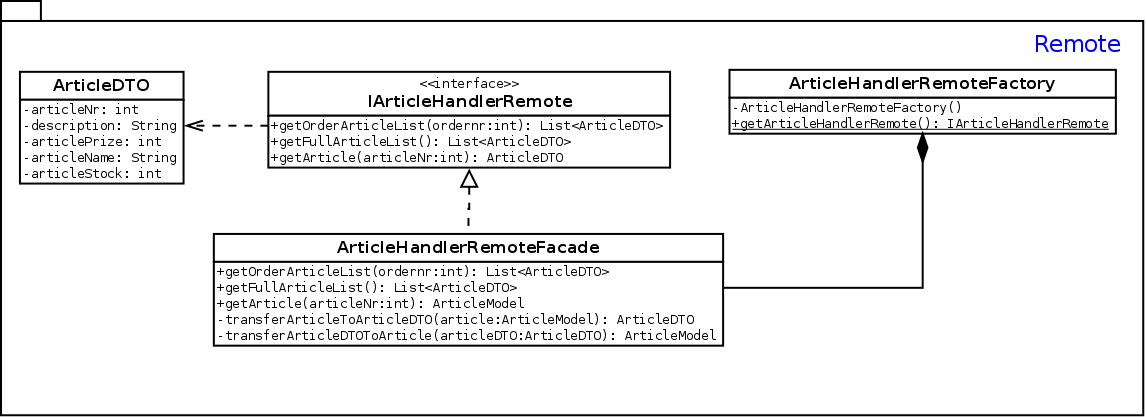
\includegraphics[width=1\textwidth]{images/classdia_article.png}
	    	\end{center}
	    \end{column}
\end{frame}
\section{Remoteschicht mit RMI}
% !TEX root = isae-beamer-template.tex

% Recall the outline at each section
\begin{frame}
  \frametitle{Remoteschicht mit RMI}
	    \begin{column}{1\linewidth}
	    	\begin{center}
	    		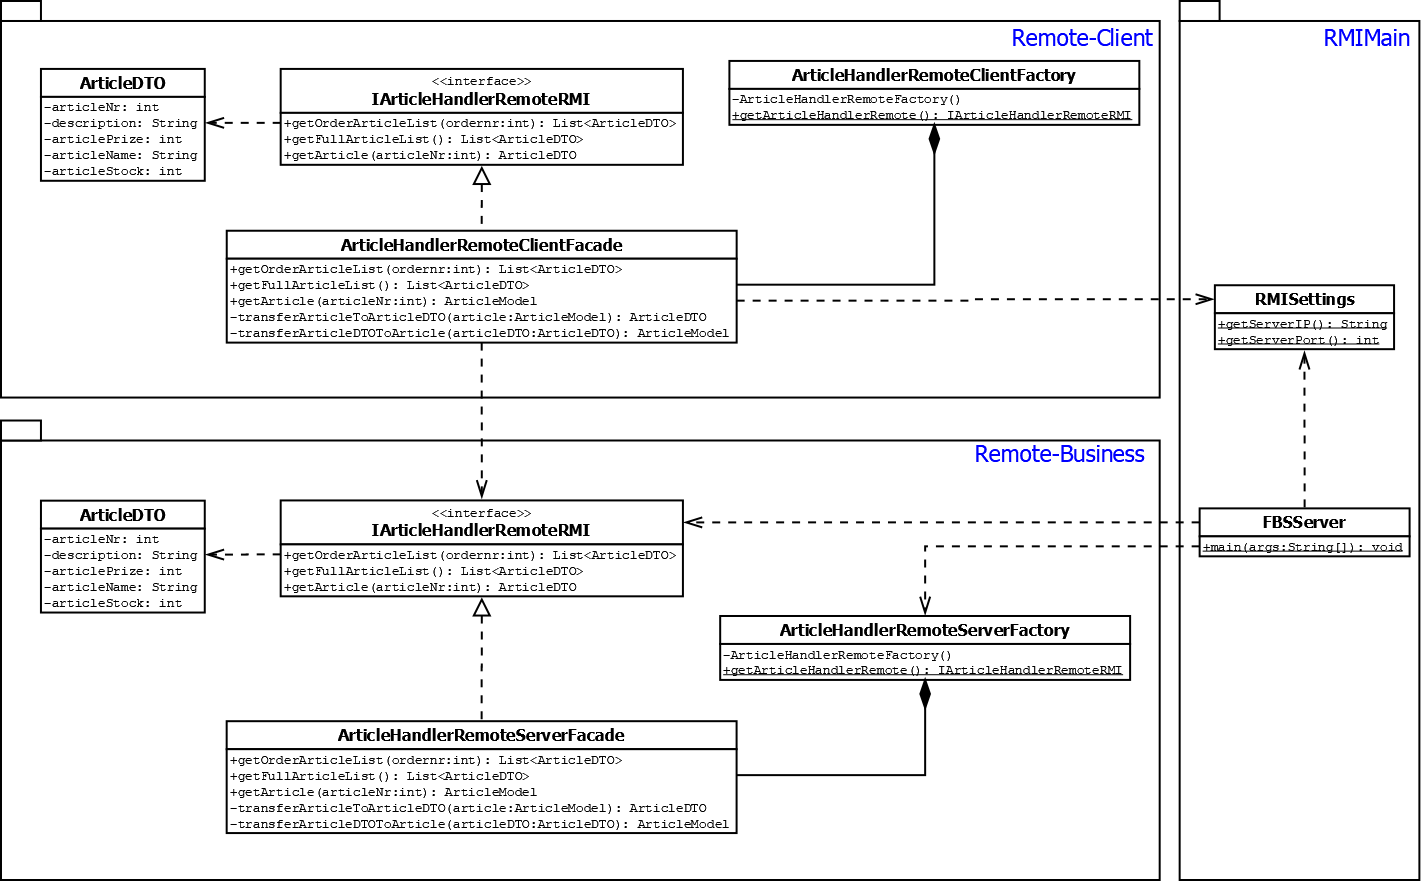
\includegraphics[width=0.8\textwidth]{images/classdia_rmi.png}
	    	\end{center}
	    \end{column}
\end{frame}
\section{Resultate}
% !TEX root = isae-beamer-template.tex

% Recall the outline at each section
\begin{frame}
  \frametitle{Resultate}
	    \begin{column}{1\linewidth}		
			\begin{center}
	    		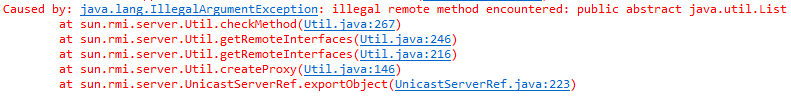
\includegraphics[width=1\textwidth]{images/Exception.png}
	    	\end{center}	
		\begin{itemize}
		\item Nur serialisierbare Typen können als Parameter und Rückgabetypen verwendet werden.
		\item Interface \textbf{List} ist nicht serialisierbar definiert.
		\end{itemize}
	    \end{column}
\end{frame}



\newcounter{lastframe}
\setcounter{lastframe}{\insertframenumber}
\setcounter{framenumber}{\thelastframe}

\end{document}
